%%%%%%%%%%%%%%%%%%%%%%%%%%%%%%%%%%%%%%%%%%%%%%%%%%%%%%%%%%%%
%%% LIVECOMS ARTICLE TEMPLATE FOR BEST PRACTICES GUIDE
%%% ADAPTED FROM ELIFE ARTICLE TEMPLATE (8/10/2017)
%%%%%%%%%%%%%%%%%%%%%%%%%%%%%%%%%%%%%%%%%%%%%%%%%%%%%%%%%%%%
%%% PREAMBLE
\documentclass[9pt,bestpractices]{livecoms}
% Use the 'onehalfspacing' option for 1.5 line spacing
% Use the 'doublespacing' option for 2.0 line spacing
% Use the 'lineno' option for adding line numbers.
% The 'bestpractices' option for indicates that this is a best practices guide.
% Omit the bestpractices option to remove the marking as a LiveCoMS paper.
% Please note that these options may affect formatting.

\usepackage{lipsum} % Required to insert dummy text
\usepackage[version=4]{mhchem}
\usepackage{siunitx}
\DeclareSIUnit\Molar{M}
\usepackage[italic]{mathastext}
\graphicspath{{figures/}}

% added by DJS 2017/01/04
\usepackage{enumitem}
\usepackage{tabularx}
\usepackage{amsmath}
%\usepackage{subfig}
%\usepackage{subfigure}
%\usepackage{subcaption}

%%%%%%%%%%%%%%%%%%%%%%%%%%%%%%%%%%%%%%%%%%%%%%%%%%%%%%%%%%%%
%%% IMPORTANT USER CONFIGURATION
%%%%%%%%%%%%%%%%%%%%%%%%%%%%%%%%%%%%%%%%%%%%%%%%%%%%%%%%%%%%

\newcommand{\versionnumber}{0.1}  % you should update the minor version number in preprints and major version number of submissions.
\newcommand{\githubrepository}{\url{https://github.com/davesmith4398/best_practice_membranes}}  %this should be the main github repository for this article

%%%%%%%%%%%%%%%%%%%%%%%%%%%%%%%%%%%%%%%%%%%%%%%%%%%%%%%%%%%%
%%% ARTICLE SETUP
%%%%%%%%%%%%%%%%%%%%%%%%%%%%%%%%%%%%%%%%%%%%%%%%%%%%%%%%%%%%
\title{Simulation Best Practices for Lipid Membranes : v\versionnumber}

\author[1*]{David J. Smith}
\author[2*]{Alan Grossfield}
\author[1,2\authfn{1}\authfn{3}]{Firstname Middlename Familyname}
\author[2\authfn{1}\authfn{4}]{Firstname Initials Surname}
\author[2*]{Firstname Surname}
\affil[1]{Department of Chemical Engineering, University of California, Santa Barbara, Santa Barbara, CA, USA}
\affil[2]{Department of Biochemistry and Biophysics, University of Rochester Medical Center, Rochester, NY, USA}

\corr{djs01@umail.ucsb.edu}{DJS}  % Correspondence emails.  FMS and FS are the appropriate authors initials.
\corr{alan_grossfield@urmc.rochester.edu}{AG}

\contrib[\authfn{1}]{These authors contributed equally to this work}
\contrib[\authfn{2}]{These authors also contributed equally to this work}

\presentadd[\authfn{3}]{Department, Institute, Country}
\presentadd[\authfn{4}]{Department, Institute, Country}

\blurb{This LiveCoMS document is maintained online on GitHub at \githubrepository; to provide feedback, suggestions, or help improve it, please visit the GitHub repository and participate via the issue tracker.}

%%%%%%%%%%%%%%%%%%%%%%%%%%%%%%%%%%%%%%%%%%%%%%%%%%%%%%%%%%%%
%%% ARTICLE START
%%%%%%%%%%%%%%%%%%%%%%%%%%%%%%%%%%%%%%%%%%%%%%%%%%%%%%%%%%%%

\begin{document}

\begin{frontmatter}
\maketitle

\begin{abstract}
%This particular document provides a skeleton illustrating key sections for a Best Practices document. Please see the sample \texttt{sample-document.tex} in \url{github.com/livecomsjournal/article_templates/templates} for additional information on and examples of using the LiveCoMS LaTeX class.
%Here we also assume familiarity with LaTeX and knowledge of how to include figures, tables, etc.; if you want examples, see the sample just referenced.

%In your work, in this particular slot, please provide an abstract of no more than 250 words.
%Your abstract should explain the main contributions of your article, and should not contain any material that is not included in the main text.
%Please note that your abstract, plus the authorship material following it, must not extend beyond the title page or modifications to the LaTeX class will likely be needed.
Here, we establish a reliable and robust standardization of settings and setup practices for practical molecular dynamics simulations of pure lipid bilayer membranes.
The simulation of lipid membranes can be a daunting task, given the uniqueness of lipid membranes relative to conventional liquid-liquid and solid-liquid interfaces, the immense and complex thermodynamic and statistical mechanical theory, the diversity of multiscale lipid models, limitations of modern computing power, the difficulty and ambiguity of simulation controls, finite size effects, competitive continuum simulation alternatives, and the desired application (including vesicle experiments and biological membranes).
These issues can complicate an essential understanding of the field of lipid membranes, and create major bottlenecks to simulation advancement.
In this document, we hope to clarify these issues, and arrive at a consistent, prioritized, and user-friendly framework for the rational design of lipid membrane molecular dynamics simulations that bridges the gap between a first-timer and world expert.

\begin{center}
	\begin{minipage}{.3\textwidth}
		\centering
		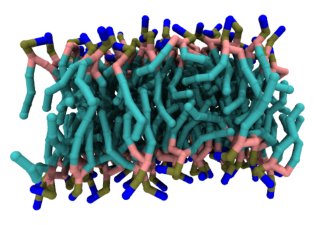
\includegraphics[width=\textwidth]{bilayer_small.pdf}
	\end{minipage}%
	\begin{minipage}{.3\textwidth}
		\centering
		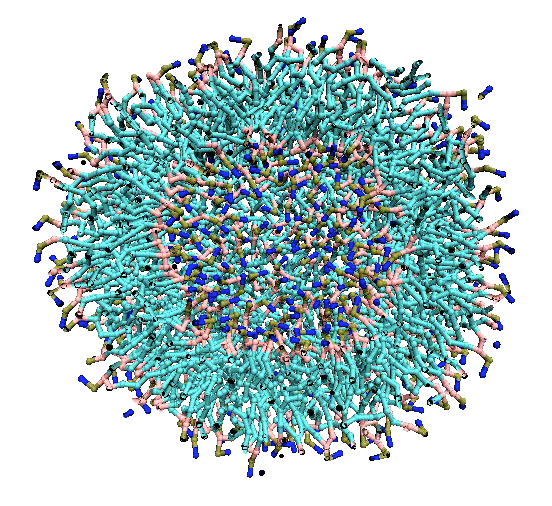
\includegraphics[width=\textwidth]{vesicle_half_small.png}
	\end{minipage}%
	\begin{minipage}{.3\textwidth}
		\centering
		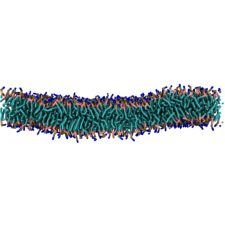
\includegraphics[width=\textwidth]{bilayer_med.pdf}
	\end{minipage}
\end{center}
%\begin{figure}[h!]
%	\centering
%	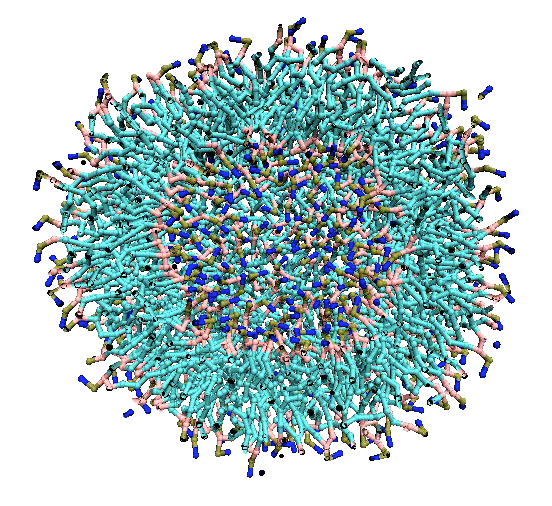
\includegraphics[width=0.5\textwidth]{vesicle_half_small.png}
%\end{figure}
%\begin{figure}[h!]
%    \centering
%    \subfloat[label 1]{{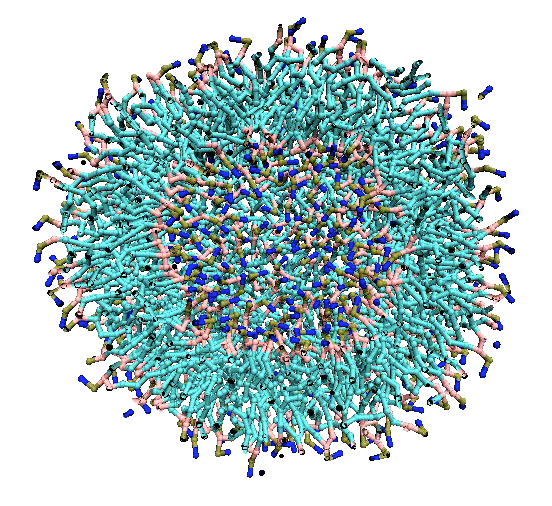
\includegraphics[width=5cm]{vesicle_half_small.png} }}%
%    \qquad
%    \subfloat[label 2]{{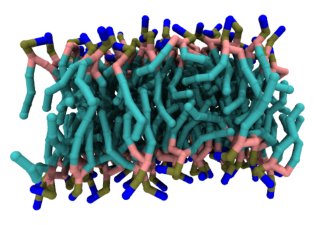
\includegraphics[width=5cm]{bilayer_small.png} }}%
%    \caption{2 Figures side by side}%
%    \label{fig:example}%
%\end{figure}
%\begin{figure}[h!]
%	\centering
%	\begin{subfigure}[b]{0.3\textwidth}
%		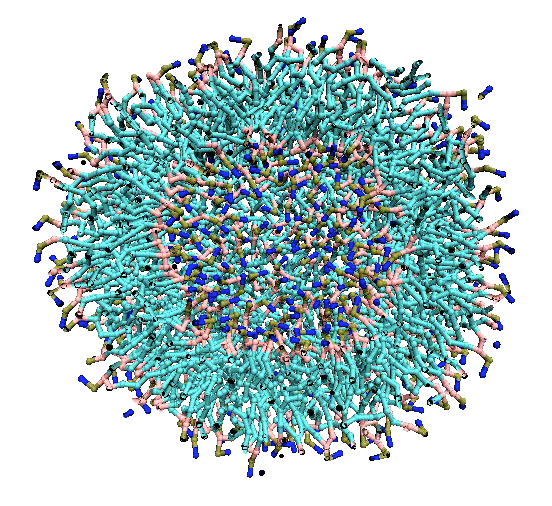
\includegraphics[width=0.3\textwidth]{vesicle_half_small.png}
%	\end{subfigure}
%	\begin{subfigure}[b]{0.3\textwidth}
%		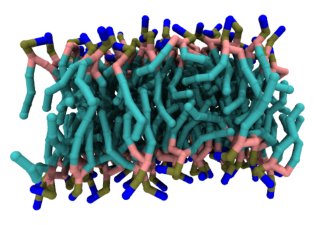
\includegraphics[width=0.3\textwidth]{bilayer_small.png}
%	\end{subfigure}
%\end{figure}
\end{abstract}

\end{frontmatter}



\section{Introduction}
%Here you would explain what problem you are tackling and briefly motivate your work.
%In this particular template, we have removed most of the usage examples which occur in \texttt{sample-document.tex} to provide a minimal template you can modify; however, we retain a couple of examples illustrating more unusual features of our templates/article class, such as the checklists, and information on algorithms and pseudocode.
Lipid bilayer membranes have diverse applications in soft matter physics, pharmacology, and consumer products, and are first approximants to biological membranes.
Lipid bilayers are quasi-two-dimensional structures consisting of two molecularly-thick layers, or leaflets, extending from nanometers to micrometers in aqueous solvent, where the roughly cylinder-shaped lipids are oriented with their polar head groups outward and their nonpolar tail groups inward.
The dominant driving forces in their formation and stability include hydrophobic and dispersion interactions, wherein the lipid tail groups maximize their contacts with each other and minimize their contacts with water, decreasing area per lipid; and head group electrostatic and excluded-volume repulsion and tail group conformational entropy, which work to increase the area per lipid [Ben-Shaul, "Handbook of Biological Physics: Chapter 7"].
Conical and inverse conical lipid amphiphiles more favorably form micelles and inverted micelles, respectively [Israelachvili, "Intermolecular and Surface Forces"].

Lamellar lipid bilayers often exist as vesicles (bilayer spheres) in solution, but can also exist as planar bilayers in periodic simulation systems and in the case of experimental supports.
Lamellar lipid membranes are interfaces embedded in three dimensions, but are more complicated than typical liquid-liquid interfaces, due to their finite thickness and preferred area per molecule [Diamant; others].
They also differ from solid-solid interfaces, due to their negligible surface tension.
Because of these complexities, simple interfacial theories of surface tension in terms of, e.g., an oil-water interface or even a fluctuating interface with capillary fluctuations are often insufficient for membranes.

Fluid lipid membranes are normally modeled as liquid-like laterally (no in-plane shear modulus), and solid-like transversely (out of plane).
Another major assumption is that the lipids are strongly surface active, and therefore are not soluble in bulk (aqueous) solvent.
The surface is consequently saturated; this achieved trivially through area relaxation in the case of tension control, and in area control, the bilayer buckles to maintain saturation.
For lipid bilayer physics, it is almost always safe to assume volume incompressibility, as negligible fluctuations in volume cost far more than typical thermal fluctuations.
Area incompressibility is a less common assumption; however, area fluctuations are often assumed to exchange with thickness (peristaltic) fluctuations through a simple equation of state (whereby area and thickness are inversely correlated) [Safran].
For this reason, a Gibbs monolayer (two-dimensional surface) description is a common and often reasonable theoretical approach.
Perhaps the most studied fluctuations in lipid membranes, and what separates them from most conventional solid-liquid and liquid-liquid interfaces, are in mesoscopic shape, termed undulations [Canham 1970; Helfrich 1973].
This is typically approached from the perspective of membrane curvature elasticity, where large wavelength bending modes are highly accessible via thermal fluctuations.
These out-of-plane modes lead to a distinction between the projected (in-plane) area and membrane contour area; therefore, care should be taken in deconvoluting deformations in membrane curvature (bending) from those in contour area (expansion/compression).
Still, other fluctuations are accessible at smaller length scales, and typically involve local lipid orientation (``tilt,'' relative to mesoscopic shape) and operations thereof, as in other liquid crystalline systems [Hamm/Kozlov; May/Narang/Kopelevich; Watson/Penev/Brown et al.].

Despite the extensive physical framework for lipid bilayer membranes from both continuum theory and experiments, detailed molecular simulations can be a tremendous asset to a further understanding.
Molecular simulations were first applied to lipid membrane systems in the early 1990s, and have since become increasingly amenable to larger spatiotemporal scales and higher resolutions [Venable, Brown, and Pastor; others].
In general, molecular simulations work well for lipid membrane studies in the following instances:
\begin{itemize}
	\item When nanometer resolution is required, and chemical detail is important (e.g. for heterogeneous membranes, and in the case of additional non-lipid components)
	\item For finite-sized systems where macroscopic thermodynamic principles may not apply
	\item For a detailed view of thermal fluctuations and the role of entropy
	\item When the interior of the membrane is being probed, and the two-dimensional/thin film assumption is not a given
	\item When bilayer self-assembly and the saturation assumption are not a given
	\item To test continuum mechanical assumptions (e.g. volume/area compressibility, tension, bending renormalization, structure of pores, etc.)
	\item To parameterize continuum theory and simulations (i.e. with spatiotemporal properties)
\end{itemize}

In any of the above conditions are met, the researcher should consider the leveraging of molecular simulations.

In the recommendations that follow, we seek to establish robust guidelines for equilibrium simulations of lipid bilayer membranes.
We focus on dilute lamellar bilayer membranes in water (i.e. at high hydration), particularly the fluid (liquid-crystalline, $L_\alpha$) phase and, where relevant, gel phases ($L_\beta$ or $L_{\beta '}$).
While we do not dictate the choice of MD package for simulation, we draw heavily on tools available in the GROMACS package, which has several built-in routines and add-on patches [FATSLiM / Buchoux. Structural bioinformatics, 2017; APL @ Voro (Lukat et al. JCTC, 2013); GridMATMD (Allen, Lemkul, and Bevan. J. Comp. Chem., 2008)] and is the default for several multiscale lipid membrane models [GROMOS 54A7 [24] in Poger, Caron, and Mark; Slipids [28] in Poger, Caron, and Mark; Marrink and Mark 2004; Marrink and de Vries 2007; Arnarez et al.].


\section{Prerequisites}
%Here you would identify prerequisites/background knowledge that are assumed by your work and your checklist which you view as critical, ideally giving links to good sources on these topics.
%Checklists are normally focused on errors made by users with training and experience in molecular simulations, so you can assume a basic familiarity with the fundamentals of molecular simulations.
Some good textbooks for statistical mechanical and thermodynamic background on membranes include:

\begin{itemize}
	\item Safran, Samuel A. ``Statistical Thermodynamics of Surfaces, Interfaces, and Membranes.'' 2003: Westview Press.
	\item Nelson, D.; Piran, T.; and Weinberg, T. ``Statistical Mechanics of Membranes and Surfaces.'' 2004: World Scientific Publishing Company.
	\item Boal, David. ``Mechanics of the Cell.'' 2012: Cambridge University Press, New York.
\end{itemize}

Good papers and textbooks for computational and simulation guidance on membranes include:

\begin{itemize}
	\item Sundararajan, V. ``Computational Modeling of Membrane Bilayers, Volume 60 (Current Topics in Membranes).'' 2008: Academic Press.
	\item Tieleman, Marrink, and Berendsen. Biochimica et Biophysica Acta, 1997.
\end{itemize}

\section{Checklist}
%Your checklist should include a succinct list of steps that people should follow when carrying out the task in question.
%This is provided to ensure certain basic standards are followed and common but critical major errors are avoided.
%Note that a checklist is not intended to cover \emph{all} important steps, but rather focus on the most common reasons for failure or incorrect results, or issues which are particularly crucial.
%Here we use a full-page checklist with multiple sections, so it will appear on a separate page of the sample PDF.
%Other checklist formats are possible, as shown in the sample \texttt{sample-document.tex} in \url{github.com/livecomsjournal/article_templates/templates}.
Here, we provide checklists for the four major steps in the lipid membrane simulation process: (1) model selection, (2) pre-simulation considerations (selection of MD settings), (3) preparation of initial configurations, and (4) post-simulation considerations (property validation).

\subsection{Model selection}
In anticipation of the final property validation, you want to first make the optimal choice of of lipid membrane model.
As with other systems, model selection for lipid membranes is crucial.
Lipid membrane models are relatively very diverse--resolution can range from all-atom to united atom to coarse-grained and from explicit to implicit solvent--and ultimately, the lipid model may be implicated in some more complicated system for the desired application (e.g. small solute transport, peptide-induced pore formation, embedded proteins).
The model selection process for a given physical problem can at times be daunting, especially for an undergraduate, experimentalist, or otherwise newcomer.
The main goal for a lipid membrane model study should be to correctly capture the correct structural, mechanical, thermodynamic, and/or dynamic properties (whatever is relevant) at the relevant length and timescales and the correct equilibrium (thermodynamic, temperature, pressure, etc.) and/or nonequilibrium (thermal/mechanical/chemical/other gradients) conditions.
However, accuracy must be optimized with efficiency.
Generally speaking, the simulation time $t_{sim}$ is a function of (1) the model, (2) the system size, (3) computing resources, and (4) MD package, amongst other factors.
These contributions are often overlapping, but can be deconvoluted in some simple scaling laws [cf. Section 4.1 for more details].
In general, force field developers seek to first capture thermodynamic properties, then address dynamical properties, as the dynamics can be tuned (e.g. via masses and thermostatting) with minimal impact on the thermodynamics.
Rigorous models are validated via their properties through experimental comparison, but with the proper corrections and normalization (most importantly, due to finite size effects in periodic simulations)[Venable, Brown, and Pastor / dynamics paper].
Transferability is ideal, but not necessarily a priority.

\subsection{Pre-simulation considerations (selection of MD settings)}
***For the sections below, good to first consult the Interfacial Systems practices, which should be consistent with this one (with major differences and nuances always noted).***
Once the model is selected, the pre-simulation considerations mainly concern the thermodynamic conditions under which the membrane simulation is ultimately going to be run.
Proper control over membrane phase behavior and mechanical tension often necessitates the use of thermostats and barostats.
As outlined in [Section 2?], the relevant thermodynamic ensembles for the study of lipid membranes are the canonical ($NVT$) and multiphase ($NP_z \gamma T$) ensembles.
NVT is appropriate for closed vesicles, due to their isotropic nature.
The multiphase ensemble (semiisotropic pressure coupling) is preferred for planar bilayers.
However, phase coexistence studies should employ NVT, as the total area for the multiphase (e.g. fluid and gel) membrane must be intermediate to the total areas of the pure fluid and pure gel membranes (with proportions of fluid and gel phase lipids determinable, e.g. via the lever rule).

The target temperature should be guided by the experimental correspondence.
For the ideal model, the simulation temperature would be set to match that of experiment.
In reality, however, the imprecise energy-entropy breakdown in the membrane model may lead to shifted phase transition temperatures, and therefore the need to simulate at a higher or lower temperature, depending on the desired membrane phase.
The main transition temperature of interest is the gel-to-liquid phase transition temperature $T_g$, above which the membrane exists in a disordered liquid crystalline $L_\alpha$ state and below which the membrane exists in an ordered gel $L_\beta$ state.
Some models may capture intermediate tilted gel $L_{\beta '}$, ripple $P_{\beta '}$, and interdigitated $L_{\beta I}$ phases whose relevance depends on the experiments you are trying to model.
Most simulations approximate a cellular membrane as a fluid lipid bilayer, and build chemical and mechanical heterogeneity in later.

For the multiphase ensemble, pressure control will additionally be required.
For membranes, pressure control is often conducted in a semiisotropic scheme, in which the $xy$ and $z$ pressures are controlled independently.
Since soft matter and biological membranes often operate at negligible tension (as their conjugate variable, the area per lipid, is unconstrained and therefore used to minimize the free energy), tensionless membranes are currently the most common.
For membranes, the definition of tension is a precarious one that might not be trivial to a newcomer.
While there is an important distinction between the frame tension $\tau$ and the Laplace tension $\gamma$, conjugate to the fluctuating membrane contour area, it has been clearly shown through thermodynamic arguments that these tensions and areas are directly related, and therefore not independent [Diamant. Phys. Rev. E, 2011.].
The Laplace tension is defined to a first approximation as:

\begin{equation}
	\label{e:partition}
	\gamma = L_z/2(P_z-(P_x+P_y)/2)
\end{equation}

Both tensions reduce to zero when the component pressures are set to be equal.

For other appropriate simulation settings, see [Section 4] and the document on general simulation guidelines (and those for interfacial systems)...

\subsection{Preparation of initial configurations}
Lamellar lipid bilayers exist for a variety of concentrations.
Certain force fields at a certain resolution normally prescribe some number of water molecules for every lipid.
For a planar bilayer, given a desired number of lipids or membrane size in the $xy$-plane can be estimated from one another if the area per lipid is roughly known:

\begin{equation}
	\label{e:partition}
	N_l = 2 L_{xy}^2/a_l \quad (planar)
\end{equation}

where $N_l$ is the total number of lipids, $L_{xy}$ is the box length is the $x$ and $y$ directions, and $a_l$ is the area per lipid. In this case, the concentration/amount of solvent can be independently varied by changing the box $z$-dimension. The number of solvent molecules can be estimated from the following:

\begin{equation}
	\label{e:partition}
	N_{solv} = L_{xy}^2 (L_z - D_B) \rho_{solv} \quad (planar)
\end{equation}

where $N_{solv}$ is the number of solvent molecules, $D_B$ is the bilayer thickness, and $\rho_{solv}$ is the estimated or known bulk density of the solvent model. Similarly, for a vesicle, the number of lipids/membrane size and amount of solvent can be estimated via:

\begin{subequations}
\begin{align}
N_l = 8 \pi R^2/a_l \quad (vesicular) \\
N_{solv} = (L_{xy}^2 L_z - 4\pi R^2 D_B) \rho_{solv} \quad (vesicular)
\end{align}
\end{subequations}

where $R$ is the vesicle radius defined from the center to the bilayer midplane.

For a vesicle, the total membrane area must be smaller than the smallest plane in periodic box; otherwise, the lipids will form a planar bilayer to minimize the free energy.
(As shown earlier, the cost of forming a vesicle from a planar membrane incurs at least a bending and Gaussian curvature energetic penalty.)
Furthermore, simulating a membrane area smaller than the smallest plane in the periodic box does not ensure the formation of a stable vesicle; in fact, a pancake structure (bilayer patch with splayed edges) is more stable up to a critical size on the order of a 10 nm radius, and therefore $10^3$ to $10^4$  total lipids! 

Once the number of lipids and solvent molecules and periodic box dimensions are determined, there are two main methods for putting them all together: (1) ``templating'' and (2) self-assembly.

In the templating method, the lipids are pre-arranged in a planar or vesicular bilayer, close to the final equilibrated structure.
Due to potential core overlaps for both planar and vesicular bilayers and the desired leaflet number asymmetry for vesicles (especially at smaller radii), existing packages and routines are recommended.
CHARMM-GUI (http://www.charmm-gui.org/) is an excellent resource, and the most common for setting up membranes in a variety of configurations and for a variety of models/force fields.
Per the general interfacial system recommendation of combining systems one at a time, the membrane can then be solvated.
Due to the fluctuating nature and molecular scale roughness of lipid membranes, a trial-and-error solvation routine may be preferred over appending solvent ?slabs? to each side of the membrane (although judgment can be used to determine which one will be more efficient).
**The GROMACS g\_solvate routine is one such example of a trial-and-error approach.**

In the self-assembly method, the lipids are dispersed in solvent, and allowed to dynamically and spontaneously arrange into their final equilibrium structure.
The proof-of-concept approach is more scientifically satisfying, but not necessarily reasonable for higher resolution models and/or larger length scale simulations due to the long time scale of assembly.
Again, care should be taken to generate a vesicle or bilayer, and not a pancake or other structure.
Because the system will always proceed to minimize its total free energy, the initial box dimensions are crucial to the outcome of the self-assembly approach.
For a planar bilayer, the in-plane box dimensions must be initialized near their intended end state (which can be predicted with the number of lipids and area per lipid), and for a vesicle, all box areas must be significantly larger than the corresponding planar bilayer with the same number of lipids (otherwise, the lipids will form a planar bilayer and not a vesicle).
For one example of the self-assembly technique, you can visit the Martini website (http://www.cgmartini.nl/index.php/tutorials-general-introduction/bilayers).

After the building step, the system should be minimized (without dynamics, at 0 K) to remove potential bad site contacts (steric overlap) generated during the original placement of molecules.
Minimization routines like steepest descent are perfectly reasonable, and are available in conventional MD packages.

Then, the system should be gradually annealed from 0 K to the target temperature in the relevant thermodynamic ensemble ($NVT$ or $NPT$, depending on whether or not a barostat will ultimately be used in the production run).
In general, a short 100 ps to 1 ns run should suffice.
The user may want to consider using position restraints during this process to prevent major lipid fluctuations, particularly if the templating method is used to initially build a bilayer.
For soft enough interactions, you may be able to skip this step.

The final preparation step involves a preliminary dynamical simulation.
In the case of templating, this is just for system equilibration in the target ensemble ($NVT$ or $NP_z \gamma T$).
A few ns should allow for relaxation of the temperature (and, if relevant, the tension), and some fluctuations about those averages.
**Just worry about main thermodynamic averages and fluctuations about them here? Even area fluctuations might take longer... [Venable, Brown, and Pastor]**
In the case of self-assembly, a longer dynamical simulation is needed to allow for bilayer formation.
For smaller (~128-lipid) membranes, this can take 10-100 ns, and can potentially take much longer for larger and vesicular ones.
Visualization can be very helpful to track the assembly process.
Care should still be taken after assembly is qualitatively confirmed to ensure quantitative equilibration.

Before the production run, the equilibrium structure can be further standardized for ease of analysis and comparison with external studies.
Out of convention, for an open planar membrane, the membrane in-plane directions are often defined to be the $x$ and $y$ directions, while the out-of-plane direction is defined as $z$.
All subsequent discussion assumes this directionality, but the choice of direction is otherwise arbitrary.
In GROMACS, this can easily be achieved with the editconf(?) command.
For both open planar and closed vesicular membranes, centering the membrane in the periodic box will largely prevent the jumping of planar leaflets and vesicle pieces across the periodic box, assuming drift does not occur.
This will make subsequent visual observation and post-simulation analysis easier.
Centering can also be achieved through editconf.

Finally, the initial estimation of the production run time is useful.
You will ultimately want to incorporate an adequate amount of sampling for your phenomenon/phenomena of interest.
In general, this means capturing several autocorrelation times for the relevant degrees of freedom.
Lipid membranes are characterized by a hierarchy of time scales, including: bond vibrations (fs-ns), trans-gauche isomerization and rotation about chemical bonds (1-100 ps), rotation (axial diffusion) about the lipid axis and wobbling (1-100ns), lateral diffusion (1-100 $\mu$s), and flip flop and undulations (1 ms-1 s) [Vermeer et al.; Konig and Sackmann, 1996; Leftin and Brown, 2011].
Collective order fluctuations (e.g. undulations, flip flop, lateral diffusion) are the longest timescale fluctuations in the system because they involve the coordination and motion of several lipids [Vermeer et al. Eur. Biophys. J., 2007.].
The time of undulations will scale as $L^4$ [Watson and Brown...].
Even at equilibrium, area per lipid can fluctuate on time scale of tens of nanoseconds [Poger, Caron, and Mark; Venable, Brown, and Pastor].
However, if your study concerns more localized or molecular degrees of freedom (e.g. rotation about chemical bonds, trans-gauche isomerization, lipid axial diffusion, etc.) at constant membrane macroscopic shape and lipid leaflet number, then smaller sampling times may be permissible.

\subsection{Post-simulation considerations (property validation)}
Fluid lipid membranes are normally modeled as liquid-like laterally (no in-plane shear modulus) and solid-like transversely.
Because of this, important properties include in-plane structure, elasticity, and dynamics and out-of-plane structure and elasticity.

Experimental reference data can be classified as either direct or indirect.
Direct data includes experimentally measured properties (e.g. x-ray and neutron form factors from scattering experiments), while indirect data includes properties inferred from direct experimental data based on a given theoretical model (e.g. area per lipid, bilayer thickness, NMR bond order parameter, lipid diffusion coefficient).
Ideally, force field and simulation validation should be based on the comparison of simulated data with direct experimental data, but this is not always possible [Poger, Caron, and Mark. Biochimica et Biophysica Acta, 2016.].
Therefore, we discuss both types of data comparisons.

Perhaps the most important verification of any lipid membrane model involves the continuous structural and mechanical profiles in the out-of-plane (``transverse'', or $z$) direction. As described earlier [Introduction? Other?], the lipid bilayer membrane's internal structure and mechanics are crucial to its physics. These metrics include (1) the local density profile and (2) the stress profile.

As for general liquid-liquid interfaces, the density profile is a crucial structural metric for lipid bilayer membranes.
Various regional models have been proposed to characterize the membrane based on its component and overall densities.
For atomistic models, the local density profile is explained by a four-region model.
The region numbering scheme proceeds from the exterior water layer to the bilayer midplane, and the typical density hierarchy is as follows: region 2 ("interface") > region 3 ("soft polymer") > region 1 ("perturbed water") > region 4 ["decane") (Tieleman, Marrink, and Berendsen. Biochimica et Biophysica Acta, 1997.]
The local density can be calculated through most conventional MD packages, although care should be taken to ensure appropriate averaging, especially for larger, more appreciably fluctuating membranes.
Be careful with programs like $g_density$ in GROMACS, which appear tabulate density averages based on absolute coordinates and not relative positions (e.g. aligning profiles each frame by the apparent membrane center).
Relative positions can be valuable when there are even minor fluctuations.
Failure to correct for this can result in smearing of the density profile; one possible outcome is that region 4 (local lipid density drop in center) is not properly captured when it should exist for a given model.
For larger membranes with significant undulations, the order parameter for the density profile (i.e. the relative z-coordinate location) must be replaced with a more appropriate one that reflects the depth into the fluctuating interface.
The local density profile can be directly compared with x-ray and neutron scattering experiments through conversion of atomic density profiles to electron and neutron density profiles, respectively, and transformation of these profiles to Fourier space.
Care should be taken here as well to account for geometric differences between planar and vesicular membranes ([Section 4]).
For AA MD data comparisons: Nagle?
Electron densities proceed generally in the same trends as above (e.g. [Klauda et al. J. Phys. Chem. B, 2010.])
What about neutrons?
For more information on techniques: Poger, Caron, and Mark...

The lateral stress profile (in the transverse direction) is a more unique mechanical metric that is highly relevant for lipid bilayers because (1) it proves whether or not your model qualitatively and quantitatively captures the competing forces in lipid bilayer assembly and stability and (2) it is the gateway to calculating a host of mechanical properties.
Despite its importance, however, the stress profile is often more difficult and expensive to calculate.
One means of calculating is through GROMACS-LS, a customized version of the MD package GROMACS.
GROMACS-LS can even calculate stress component profiles, including those arising from van der Waals and electrostatic interactions.
For more information about package and theory: http://mdstress.org/ [Ollila et al.; OTHERS].
As an important verifying metric of force field development, the stress profile can be thoroughly compared with existing atomistic simulation studies.
There is no direct means of stress profile comparison with experiments, though as we will explain, properties calculated from the stress profile can be compared with experiment (cf. mechanical properties...).

The membrane thickness is a structural metric that is consequently calculated from the density profile. Two experimentally-relevant definitions include (1) the Luzzati (total lipid) thickness $D_B$ and (2) the head-to-head distance $D_{HH}$.
The Luzzati thickness is relevant to neutron scattering, and is calculated as the distance between the two locations on each side of the bilayer where the water density drops to one half its bulk value.
This thickness metric in reality is based on the spatial profile of protiated and deuterated water, and is physically indicative of the degree of water penetration into the bilayer [Poger, Caron, and Mark].
The head-to-head distance is relevant to x-ray scattering, and calculated as the distance between the two peaks in the electron density profile.
More simply, this can also be approximated as the distance between the maximal phosphate group densities in each leaflet (relevant to coarser lipid models) [Poger, Caron, and Mark].
Both can be indirectly compared with experiment.
For comparison, the experimental results are typically converted to real space.
Typical values for phospholipid bilayers in simulation and experiment are around 4 to 5 nm [REFs].

Two important structural parameters, complementary to one another, are (1) the area per lipid (providing information about in-plane structure) and (2) the deuterium NMR order parameter (for out-of-plane structure).

The area per lipid, or in-plane area occupied by a given lipid, is another critical target in force field parameterization of lipid membranes [Venable, Brown, and Pastor, 2015].
In simulation, the area per lipid is typically calculated via

\begin{equation}
	\label{e:partition}
	a=(L_x L_y)/n
\end{equation}

where $L_x$ and $L_y$ are the lateral box dimensions, and $n$ is the number of lipids per leaflet [Poger, Caron, and Mark].
This equation assumes a lipid number symmetric bilayer with negligible undulations, such that the contour (membrane) and projected (periodic box) areas are roughly equal [Venable, Brown, and Pastor, 2015].
However, for larger membranes, undulations will lead to significant differences between the contour and projected areas.
Theoretically speaking, undulations will increase the ratio of contour area to the projected area, and this is specifically because the undulations reduce the projected areas [Venable, Brown, and Pastor, 2015; Braun et al.].
The area per lipid is rigorously an intensive, or size-independent, quantity (cf. theory..), so the appropriate steps should be taken to normalize for significant size effects when necessary before experimental comparison.
This may warrant simulation of different membrane sizes, extrapolating results to zero system size to allow for convergence of contour area to frame area and arriving at a size-independent metric [Waheed and Edholm].
However, the area per lipid may not vary much across typical sizes of MD simulations, or even in experiments [cf. Theory].
In any event, care should be taken to ensure proper statistics.
Even at equilibrium, the area per lipid can fluctuate on a time scale of 10-100 ns [Poger, Caron, and Mark].
For multicomponent membranes, the membrane should be partitioned into individual values for each lipid species (cf. Voroni tessellation-based methods, grid-based methods using atomic van der Waals radii, etc.).
Partial molar areas can be determined, but this requires that a range of concentration ratios be simulated.
For more information, see: REF.

The deuterium $P_2$ NMR order parameter describes the alignment of lipid constituent bonds with the global membrane normal, and will vary along the length of the lipid tail group chains, and between liquid crystalline and gel phase lipids.
The metric is defined as:

\begin{equation}
	\label{e:partition}
	S_{CD}=1/2<3cos^2\theta-1>
\end{equation}

A value of 1 indicates perfectly alignment of the chain with the global bilayer normal, while -0.5 indicates anti-alignment.
This metric, however, can be ambiguous.
For example, a value of zero can mean either that the lipids are isotropically disordered with respect to the bilayer normal, or that the lipids are perfectly oriented at a constant angle equal to the ``magic angle'' of 54.74$^{\circ}$ [Poger, Caron, and Mark].
Computing error bars is tricky, but the order\_parameters tool in LOOS offers one approach.
Since area per lipid and the NMR order parameter are tightly coupled, a similar magnitude of statistics is required for $S_{CD}$ as well.
Calculated metrics can be compared with other simulations and indirectly with quadrupolar NMR splitting experiments.
From the top of the acyl chains to the bottom, values typically rise from ~0.17-0.20, then fall from around ~0.20-0.22 to ~0.10 for a fluid phase phospholipid bilayer.
Averages across the entire chains are therefore typically around 0.17 [Venable, Brown, and Pastor].

The area per lipid can be compared directly with other simulations and indirectly with experiments.
For simulation comparison, normalized size-independent metrics should be obtained where possible.
The area per lipid cannot be measured directly experimentally, due to the complications of lateral and transverse structure fluctuations, but the area per lipid is usually inferred from a theoretical model.
One example uses the lipid volume $V_L$ and the Luzzati thickness: $a=2V_L/D_B$.
This assumes, however, that the lipid volume can be estimated accurately [Poger, Caron, and Mark].
Another approach uses the deuterium NMR order parameter: $a/chain=2V_{CH_2}/((1+2S)b_{cc})$, where $S$ is the plateau value of $S_{CD}$ (see below for details) and $b_{cc}$ is projected C-C bond length along bilayer normal [Nagle 1993].
Practically speaking, these comparisons are difficult because $S_{CD}$ contains contributions from conformational disorder, local lipid tilting, and assorted collective motions [Venable, Brown, and Pastor, 2015].
The value for double-tailed phospholipids is generally larger than single-chain hydrocarbons in systems like SAMs (60 \AA$^2$/molecule as opposed to 30-40 \AA$^2$/molecule) [REFs].

The lipid lateral diffusivity $D_l$ is used to characterize lipid mobility, to gain insight into collective lipid motion timescales, and also potentially to discriminate between liquid crystalline and gel phase lipids.
The relevance of a diffusivity is predicated on the assumption of classical in-plane diffusion.
As such, the diffusivity can be determined from the slope of the average lipid mean-squared displacement (MSD) plotted against lag time (equal to $4D_l$ for 2D diffusion).
In the MSD calculation, the user should be careful of artifacts due to lipid molecules partially or fully jumping across periodic boxes; periodicity can be accounted for by reimaging where appropriate.
For homogeneous, single-component lipids, averages are normally taken over all lipids.
Results typically call around O($10^{-8} to 10^{-7} cm^2/s$.
Simulation results can vary significantly with the force field, system size, truncation scheme for long-range interactions, time step, and non-bonded interaction pair list update frequency [Poger, Caron, and Mark].
Venable et al. recommends that, when reporting and comparing with other simulations, the system size in particular should be noted and accounted for.
Given the hydrodynamic theory, the lateral and transverse dimensions would be even more explicit, and ideally, studies should report extrapolated infinite size values with a confidence interval [Venable et al. J. Phys. Chem. B, 2016.].
Results can be indirectly compared with experiment.
Experimental estimates can generally vary over three orders of magnitude, due to a number of reasons [cf. Section 4 for more details] [Venable et al.].

Mechanical properties for membranes can be calculated from a number of techniques that can be broadly classified by (1) equilibrium fluctuations, (2) stress profile, and (3) biased/active deformations.
We discuss the merits of each umbrella of approaches in general terms in [Section 4].
In this section, we merely attempt to recommend the best technique(s) for a given property.
These mechanical properties include: (1) lateral tension, (2) area compressibility modulus, (3) bending modulus, (4) monolayer spontaneous curvature, (5) Gaussian curvature modulus, and (6) line tension.

(1) Calculation of the lateral tension from a membrane simulation is a way to calculate the variable conjugate to the membrane [contour] area in canonical simulations, and in tension control, a way to directly confirm the simulations controls for the intended ensemble.
In model development, the tension is a parameter probed to capture the correct area per lipid (which should ideally occur at zero tension) [Zgorski and Lyman].
The tension is related to the zeroth moment of the stress profile, and can be easily approximated with the Kirkwood-Buff equation [cf. Section 3.2 above].

(2) The area compressibility modulus determines a membrane's ability to compress and expand, and is another important property in force field parameterization [Venable, Brown, and Pastor, 2015].
The recommended way to calculate $K_A$ is based on area fluctuations in the tensionless ensemble:

\begin{equation}
	\label{e:partition}
	K_A^{app} = k_BTA_p/\sigma_{A_p}^2
\end{equation}

where $K_A^{app}$ is the apparent area compressibility modulus based on the fluctuations in lateral box dimensions.
This equation is fairly simple, but involves two major nuances.
The first is that the calculation may take up to 100 ns to converge [Venable, Brown, and Pastor, 2015].
The second is that this is an apparent value based on size-dependent projected area fluctuations, and is not the end point for characterizing the intensive, size-independent in-plane compressibility.
The recommended correction to deconvolute expansion-compression modes from undulatory modes is to simulate multiple membrane sizes and extrapolate the results to zero system size, where undulations no longer exist [Waheed and Edholm].
At smaller simulated system sizes, the result of not accounting for undulatory contributions can be negligible (~5-10\% correction with experiment), but becomes substantial and must be corrected for larger system sizes (where they can be ~50\% larger than experimental results) [Waheed and Edholm; Venable, Brown, and Pastor].
Results typically vary between 100 and 400 mN/m [CONFIRM? REFS?], and are often compared with micropipette aspiration experiments [Rawicz et al., 2000].
Results can also be compared with predictions from polymer brush theories, where $K_A$ is sometimes related to the oil-water interfacial tension $\gamma^{o/w}$ [Seth et al.; others]--for example, $K_A = 6 \gamma^{o/w}$ [Rawicz et al. Biophys. J., 2000].

(3) The bending modulus (bending rigidity/constant) determines the ability of the membrane to bend.
The undulation spectrum method [Goetz et al. PRL, 1999; Lindahl and Edholm. Biophys. J., 2000] is the traditional and well-established way to calculate $\kappa$.
The spectrum describes the height-height correlations of the membrane continuum shape, and for a tensionless membrane, the large wavelength/small wavevector behavior follows an inverse fourth power relation with a constant of proportionality that contains the bending modulus [Goetz et al. PRL, 1999; Lindahl and Edholm. Biophys. J., 2000]:

\begin{equation}
	\label{e:partition}
	<|h_q|> = k_BT/\kappa q^4
\end{equation}

The undulation spectrum method, however, must be used over "mesoscopic" length scales (approximately ten times the bilayer thickness, or about 50 nm / 5000 lipids) that are out of reach for AA and most CG simulations.
If simulations are too small, deviations to the undulation spectrum will result from individual lipid tilting (below ten thicknesses) and protrusions (below three thicknesses) [Venable, Brown, and Pastor].
Also, there will simply not be a large enough range of wave vector magnitudes to fit the spectrum and obtain a bending modulus estimate.
For this reason, we recommend the lipid director field spectrum approach [Watson et al., 2012; Venable, Brown, and Pastor; others], which analyzes thermal fluctuations of lipid orientation via a director vector field $\hat{n}$.
Specifically, the longitudinal component of $\hat{n}$ relates to the macroscopic bending modulus through an inverse second power relation in the wave vector:

\begin{equation}
	\label{e:partition}
	<|\hat{n}_q^{||}|> = k_BT/\kappa q^2 \quad (recommended)
\end{equation}

The lipid director field spectrum method works well for "modestly-sized" membranes, down to approximately three bilayer thicknesses (~12-15 nm); AA simulations of 648 lipids have been shown to be well converged.
This general approach also provides a route to calculating bilayer tilt and twist moduli.
Both the undulation and lipid director field spectrum approaches will take at least 100 ns to converge [Venable, Brown, and Pastor, 2015].
Technically speaking, the bending modulus is not a material property; it is dependent on system size, and decreases at larger scales as $\kappa[\lambda] = \kappa _0 - 3k_BT/4\pi ln(\lambda a)$ [Peliti and Leibler; Deserno; others].
The determination of the appropriate size renormalization is somewhat ambiguous, but the length scale of the relevant experimental system can be used as a guide.
Bending modulus results typically vary between 10 and 40 $k_BT$ [CONFIRM? REFS?], and can be compared with a host of experimental techniques, including flicker spectroscopy and micropipette aspiration [cf. Section 4 for more details].
Results can also be compared with polymer brush theory, which relates $\kappa$ to $K_A$ and the bilayer hydrophobic thickness via $\kappa = K_Ah^2/24$ [Evans...].

(4) While lipid bilayers (planar and vesicular) have a net zero bilayer spontaneous curvature $C_0$, their monolayers individually may have a propensity to curve.
This propensity is quantified by the monolayer spontaneous curvature $c_0$, and is defined to be positive for a lipid that forms micelles and negative for one that forms inverted micelles [Venable, Brown, and Pastor].
Together with the monolayer bending modulus $\kappa_m$, $c_0$ is related to the first moment of the stress profile, integrated from the bilayer midplane to the upper edge of the simulation cell [Safran, 1994]:

\begin{equation}
	\label{e:partition}
	\kappa_m c_0 = \int_{0}^{L_z/2} z[P_xy(z) - P_z]dz
\end{equation}

Thus, if $\kappa_m$ is known, then $c_0$ can be quantified.
$\kappa_m$ is predicted by elastic theory to be one half the bilayer value ($\kappa$).
Monolayer spontaneous curvatures are typically calculated indirectly in experiment from studies in the completely different inverted hexagonal $H_{II}$ phase, where lipid monolayers are assmembled in long, hexagonally-arranged water-filled tubes.
Results are then extrapolated to the lamellar phase.
This is hard to study for lipids like DPPC that are more cylindrical in shape, but easier for those like DOPE that are more like inverted truncated cones (due to acyl chain unsaturation) [Venable, Brown, and Pastor; Israelachvili].

(5) The Gaussian curvature modulus describes the propensity of the membrane to change topology, and is especially important for fission and fusion events [Hu, Briguglio, and Deserno. Biophys. J., 2012].
In general, even simulation methods for calculating $\kappa_G$ are controversial.
The difficulty in calculating $\kappa_G$ lies in controlling topology and boundary behaviors in which Gaussian curvature plays a role [Hu et al.].
The stress profile approach, specifically involving the second moment, is not reliable here [Hu et al. 2012, 2013].
We recommend the patch closure method, which has shown promise in preliminary work [Hu, Briguglio, and Deserno. Biophys. J., 2012].
While there is virtually no means for experimental comparison, elasticity theories offer simple predictions, particularly in the approximation $\kappa_G \approx -\kappa$ [Deserno. Macromol. Rapid Commun., 2009; Hu, Briguglio, and Deserno; Ramakrishnan et al.].

(6) A line tension (edge energy) is an energy per unit length that can describe lipid phase segregation and hole formation.
Specifically for pores (hydrophilic holes, where lipids splay to connect the two leaflets), the line tension can be studied through simulation of a bilayer "strip" or "half-connected bilayer" (with exposed bilayer edges in one in-plane box dimension).
The bilayer is thus periodic in one lateral dimension and exposed in the other, resulting in lipid splaying and therefore a rim on both sides.
In this scenario, the line tension can be determined from the stress profile, specifically the lateral normal stresses.
If the strip is periodic in $y$ and non-periodic in $x$, then:

\begin{equation}
	\label{e:partition}
	\Gamma = 1/2 L_x L_y (P_{xx} - P_{yy})
\end{equation}

and $P_{xx} = P_{zz}$ [Tolpekina, den Otter, and Briels. J. Chem. Phys., 121, 8014, (2004).].
Typical values are around 35 to 50 pN in simulation [Tolpekina, den Otter, and Briels; Wohlert, den Otter, Edholm, and Briels] and 5 to 30 pN in experiment [Brochard-Wyart et al.; Moroz and Nelson; Zhelev and Needham; Evans, Ludwig, and Florian; Loi et al.], the latter of which are typically through dynamical pore closure studies.

While thickness, area per lipid, deuterium order parameter, and lipid lateral diffusivity calculations do not necessarily require leaflet identification, other metrics do. Leaflet identification and the relevant metrics are discussed in [Section 4].

The method of calculation in experiment does matter to the method of calculation in simulation.
For example, methods based on biased membrane perturbations may deviate significantly from those based on equilibrium fluctuations (e.g. micropipette aspiration versus flicker experiments) [Venable, Brown, and Pastor, 2015].
Wherever possible, the theoretical basis for both the experimental and simulation property calculations should be used as a guide.

A final point is that experimental results are not infallible.
When simulation and experiment do not agree and one is fairly confident in the simulation procedure and results, the experimental results can be questioned [Venable, Brown, and Pastor, 2015].


% This provides a checklist which
% - spans a full page
% - consists of multiple sub-checklists
% - exists on a separate page
% This style of checklist will be especially helpful if you want to encourage readers to print and use your checklist in practice, as they
% can easily print it without also printing other material from your manuscript. However, other styles of checklist are also possible (below).
\begin{Checklists*}[p!]

\begin{checklist}{1. Model Selection}
\textbf{Goal: set up model to accurately capture properties of interest in an efficient manner.}
\begin{itemize}
\item Lay out problem/phenomenon of interest, and establish whether or not molecular simulations are needed.
\item If molecular simulations are needed, determine:
	\begin{itemize}
	\item Available computing resources (cores, memory, etc.)
	\item Desired lamellar membrane configuration (planar vs. vesicular)
	\item Overall relevant length and time scales of the system of study (or, if possible, of an appropriate subsystem)
	\item Primary properties of interest (structural, mechanical, thermodynamic, and/or dynamic)
	\item Required spatiotemporal resolution
	\end{itemize}
\item Based on the above considerations, determine the optimal model in terms of accuracy and efficiency.
\item Items in your checklist can and should reference sections where the cited issues are discussed in detail, such as Section~\ref{sec:reference_this}
\end{itemize}
\end{checklist}

\begin{checklist}{2. Pre-Simulation Considerations (Selection of MD Settings)}
\textbf{Goal: establish rational and physically-intuitive settings for the desired lipid membrane simulation.}
\begin{itemize}
\item Determine desired thermodynamic ensemble.
\item Given selected model and experimental correspondence, determine target temperature.
\item If relevant, determine pressure control settings.
\item Determine remaining settings necessary for MD configuration file.
\end{itemize}
\end{checklist}

\begin{checklist}{3. Preparation of Initial Configurations}
\textbf{Goal: build reasonable equilibrium starting structure for a lipid bilayer in a periodic simulation box.}
\begin{itemize}
\item From the desired membrane size, estimate the number of required lipids.
\item From the desired concentration, estimate the number of solvent molecules and periodic box dimensions.
\item Using the above estimates, proceed through the system setup:
	\begin{itemize}
	\item Method A: Templating: build membrane, solvate
	\item Method B: Self-Assembly: insert lipids, solvate
	\end{itemize}
\item Minimize (no dynamics) to remove bad site contacts
\item Anneal from 0 K to target temperature
\item Dynamics
	\begin{itemize}
	\item Method A: just equilibrate
	\item Method B: self-assemble, then equilibrate
	\end{itemize}
\item Qualitatively confirm equilibrium structure and quantitatively confirm thermodynamic averages.
\item Rotate/re-center system as necessary.
\item Determine reasonable amount of sampling for production run.
\end{itemize}
\end{checklist}

\begin{checklist}{Simulation Production Run}
\end{checklist}

\begin{checklist}{4. Post-Simulation Considerations (Property Validation)}
\textbf{This is some further description.}
\begin{itemize}
\item Calculate and validate density profile via scattering form factors, and if possible, calculate stress profile.
\item Calculate and validate thickness, area per lipid, deuterium NMR order parameters, and lipid lateral diffusivity.
\item Calculate and validate mechanical properties as necessary. If required, set up and run additional simulations for certain properties.
\item Determine if leaflet identification is necessary for other metric calculations. Proceed as necessary.
\end{itemize}
\end{checklist}

\end{Checklists*}





\section{Rationale}

Your Rationale section, or sections, can follow or precede your checklist (we expect that often, following the checklist will be preferable) and provide the necessary rationale for the checklist, and act as more complete \emph{best practices} description.
This should include 1) significant detail as to the possible alternative ways to accomplish a given task, 2) description of advantages and disadvantages of the various approaches, and 3) significant literature documentation about reasons for choices.

\subsection{Model selection}
Efficiency is a major concern in virtually any lipid membrane simulation.
In the MD loop, the most expensive step involves the pairwise force evaluations, and therefore the number of particles in your system $N$ and the system density $rho_{model} ~ 1/a_{model}^3$, where $a_{model}$ is the average spacing between sites in the model [cf. other Docs; Shell. Thermodynamics and Statistical Mechanics: An Integrated Approach.]
Exact $t_sim$ scalings depend on the force field, and can range from $N \rho$ for short-ranged/mean field types of force fields to $NlogN$ (e.g. PME) to $N^2$ for long-ranged/rigorous pairwise interactions.
Since the number of particles can be related to the system density $rho_{model}$ and the system length scale $L$ (e.g. cubic box):

\begin{equation}
	\label{e:partition}
	N = \left\{
        		\begin{array}{ll}
            		\rho L^3 & \quad (explicit solvent) \\
            		\rho L^2 & \quad (implicit solvent)
        		\end{array}
    	\right.
\end{equation}

this scaling partly incorporates the model resolution $rho_{model}$ and system size $L$/nature of solvent, respectively.
For example, for short-ranged interactions:

\begin{equation}
	\label{e:partition}
	t_{sim} \propto \left\{
        		\begin{array}{ll}
            		\rho^2 L^3 & \quad (explicit solvent) \\
            		\rho^2 L^2 & \quad (implicit solvent)
        		\end{array}
    	\right.
\end{equation}

and for long-ranged:

\begin{equation}
	\label{e:partition}
	t_{sim} \propto \left\{
       		 \begin{array}{ll}
            		\rho^2 L^6 & \quad (explicit solvent) \\
            		\rho^2 L^4 & \quad (implicit solvent)
        		\end{array}
    	\right.
\end{equation}

There is additionally a system size contribution in addition to the geometric one that accounts for sufficient sampling.
This accounts for the largest wavelength undulations that are the slowest degree of freedom, and scales as $L^4$ [Watson and Brown. Biophys. J., 2010.].
Thus, the overall scaling in system size can be from $L^6$ up to $L^10$, depending on the range of interactions and presence/absence of solvent.
In other words, at a minimum, an order of magnitude increase in membrane length scale leads to six order of magnitude increase in computational expense!
Furthermore, coarser models may contribute to higher accessible time scales in two ways: (a) by increasing the time scale of the fastest (vibrational) mode (i.e. $t_{sim} ~ 1/\Delta t_{model}$) and (b) by also inherently smoothening the free energy landscape, and therefore enhancing dynamics across it (e.g. via a simple scale factor).
Computing resources and the specific MD package can be viewed as (a) affecting the range of possible parallelization schemes (described in speedup by, e.g. Amdahl's Law, but convoluted with the specific MD scheme, e.g. domain decomposition) and (b) contributing to some intrinsic scale factor related to the hardware type (e.g. CPUs vs. GPUs) and software type.

In general, there is a very diverse range of models that can be leveraged for simulations of lipid bilayer membranes.
Atomistic (all-atom, or AA) models are the ``gold standard,'' as is the case with MD simulations of most other systems.
The quality of AA MD simulations of lipid bilayers has improved dramatically since their initial development in the early 1990s [Venable, Brown, and Pastor. Chemistry and Physics of Lipids, 2015].
AA models can have hundreds of atomic sites per lipid molecule.
Little more on AA MD?
United atom (UA) force fields remove hydrogen atoms for an increase in efficiency (NUMBER?), and are becoming competitive with AA force fields in accuracy.
Little more?
AA and UA can therefore typically reach 10 to 100 ns time scales and 5 to 10 nm length scales [Smirnova et al.].
Well-validated force fields include AMBER Lipid14 (AA??) [26], CHARMM36 (AA) [27], GROMOS 54A7 (UA) [24], and Slipids (AA) [28; all in Poger, Caron, and Mark!].

Coarse-grained (CG) models have also been well-developed for efficient, large-scale simulations of lipid membranes, often where the interest is in mechanical and qualitative behaviors and less in the quantitative and chemical detail.
That said, systematic CG models can still retain some level of chemical specificity (e.g. the types of lipids that they represent).
CG models can reach 100 to 1000 ns (1 $\mu$s) time scales and 10 to 20 nm length scales [Smirnova et al.].
One of the best-known CG models for membranes is the Martini force field [Marrink and Mark 2004 and 2007 papers], which via a 4:1 heavy (non-hydrogen) atom mapping can have around ten pseudoatom sites per lipid. Martini is a hybrid bottom-up and top-down method of coarse-graining, combining nonbonded interactions parameterized to capture experimental partitioning free energies and bonded interactions parameterized from AA simulations [Marrink and Tieleman. Chem. Soc. Rev., 2013].
Because the aqueous solvent can contribute up to 90 percent of the force evaluations [Arnarez et al.; Baukina, Marrink, and Tieleman. Biophys. J., 2012], implicit solvent (IS) simulations can be much more efficient and potentially advantageous as well.
The Dry Martini force field [Arnarez et al.] is one of many such examples, and offers a factor of between 2 and 100 speed-up relative to conventional (``wet'') Martini [Arnarez et al.].
There are many other examples of both explicit [REFs?] and implicit [REFs?] solvent CG models for lipid membranes.
However, CG models in general and IS CG models in particular are sometimes deficient in capturing solvent-mediated effects, entropic driving forces, and hydrodynamics.
The wet Martini model in particular has paired lipids with many different types of CG water models; successive models incorporate crucial features like polarity, but at the expensive of computational efficiency.
With the intuition that the effective thermodynamic properties are already well captured with IS CG Martini, recent work has sought to improve dynamical properties via a hydrodynamics thermostat, with minimal computational overhead to model the solvent (about a factor of four increase in efficiency relative to the corresponding explicit solvent model) [Zgorski and Lyman].

Phenomenological, generic, and toy models work more in a top-down fashion by incorporating and tuning minimalistic interactions to obtain the desired phenomena and properties.
Examples include IS CG models that have been further developed with five [Brannigan, Philips, and Brown. Phys. Rev. E, 2005] and three [Cooke and Deserno. J. Chem. Phys., 2005] sites, and recent efforts have sought to incorporate hydrodynamic thermostatting here as well [Atzberger].
These models extend the range of accessible scales even further to 10-100 $\mu$s and 10-100 nm [Smirnova et al.].
These types of simulations have executed as low as two- or three-site lipid models in conjunction with a dissipative particle dynamics (DPD) thermostat (i.e. DPD simulations).
Practically speaking, only two sites per lipid are needed (one hydrophilic and one hydrophobic) to capture amphiphilicity and consequently self-assembly into lipid bilayers.

For lipid membranes, there is also an extensive sub-community that uses continuum mechanical theory and field-theoretic simulations that are sometimes in fact the preferred approach at larger length scales (100 nm to 100 $\mu$m) due to their efficiency [Smirnova et al.; Brown Annu. Rev. Phys. Chem.].
Simulations are performed on the basis of the above continuum theoretical descriptions and by parsing different deformation modes and perturbing them, accepting or rejecting perturbations based on a Metropolis criterion [Cray? Brown. Maibaum].
It is often crucial to compare with these techniques wherever possible.
If some of these above conditions motivating the use of molecular simulations are not met, it is useful to evaluate whether or not a continuum approach would be better.

It should be evident from the thermodynamic and statistical mechanical framework above that there are some crucial considerations for any lipid membrane model, regardless of resolution, including: (1) membrane composition, (2) other thermodynamic constraints, and (3) the model dimensions.

In terms of composition, it is generally important to consider the chemical mapping of the model to the real system, especially for multicomponent membranes.
The desired heterogeneity and lipids in particular may determine the model you ultimately choose.
In lipid membrane simulations (for both atomistic and coarse-grained resolutions), the canonical system is DPPC (dipalmitoylphosphatidylcholine) in water.
DPPC is a lecithin, a common choice for vesicle experiments, and a major component of pulmonary surfactant.
This is typically the system for which new force fields are first tested.
DPPC is sometimes not preferred in experiments, however, due to its high melting point (from the gel to liquid-crystalline state).
In fact, for biologically-relevant simulations, we advise caution in the selection and relative composition of lipids in the membrane model.
While there are good guidelines for the contributions of major lipid head and tail groups to biological membranes, composition can potentially vary across different domains and even between two leaflets [Ing\'olfsson et al. ``Lipid organization of the plasma membrane.'' JACS, 2014], and the best choice for a given model will depend highly on the analogous experimental system.

Given a membrane's composition, the thermodynamic constraints of temperature and tension (or area) will largely determine phase behavior.
As discussed above, simulations are sometimes amenable to different constraints from experiments, but the appropriate experimental conditions can be achieved in a corresponding simulation ensemble.
It is worth noting that certain models, particularly CG ones, sometimes experience difficulty in capturing phase transition temperatures and even entire phases (for example, subgel and ripple for Martini)[Smit].

Whether or not the membrane physically reflects the experimental setup also depends largely on the dimensions of the model.
It has been shown for membranes that finite size effects can play a significant role for thermodynamic (especially mechanical) and dynamical properties [Feller et al.; Castro-Rom\'an et al.; Waheed and Edholm; Venable et al.; etc. etc. etc.].
This refers not only to the in-plane dimensions, but also for the out-of-plane one; despite the quasi-two-dimensional structure of membranes and two-dimensional approximation at larger length scales, hydrodynamic theoretical models for periodic systems have shown that the thickness of the water layer(s) matter as well in convergence to macroscopic dynamics [Venable et al.].
In determining the model dimensions, one should search for the emergent length scales in the experimental system that can serve as the periodicity length scales in the simulation.
For biological membranes, there is experimental evidence to show that an appropriate in-plane length scale is around 150-500 nm.
This is set by the cortical cytoskeletal mesh, which pins membrane proteins and therefore constrains lipid motion (anchored protein picket model) [Ritchie et al. Molecular Membrane Biology, 2003; Morone et al. J. Cell Biology, 2006].
This is too large for most molecular simulations, but if a highly resolved picture of biological membranes is still desired, different subsystems can be simulated.
If you're not going to simulate the experimentally relevant size (of the overall experimental system or a relevant subsystem), then you need to be able to normalize your results with respect to the different sizes.

A final point is on comparison of different geometries.
In many cases, experimental vesicles are modeled with planar bilayer simulations.
This may raise questions about the meaning of the results, as vesicular membranes are the result of a balance of positive strain on the outer leaflet and negative strain on the inner leaflets, while planar membranes have on average zero strain on each leaflet.
Furthermore, vesicles often have a different number of outer and inner leaflet lipids.
Rigorously speaking, there are mathematical transformations to convert data between vesicles and the corresponding planar bilayer
However, large enough vesicles are also locally flat, and their extensivity can be used as a guide for the simulation size (or the size to which you normalize your results).

\subsection{Pre-simulation considerations (selection of MD settings)}

Technically, NVE (pure MD) is the correct ensemble for all MD simulations, and is strictly the only ensemble in which pure dynamics are observed [cf. general guidelines].
To roughly conserve energy and prevent drift, the integration settings (time step, etc.) matter.
Since periodic center of mass removal can hide integrator artifacts, removal should ideally only occur at the start of the simulation [Zgorski and Lyman].
However, as mentioned earlier, proper control over membrane phase and tension often necessitates the use of thermostats and barostats.
In some cases, this (as well as the long-range electrostatic calculation method) can lead to significant drift when the center of mass motion is not removed [Zgorski and Lyman].
It has been shown, however, that weak-coupling thermostats and barostats and periodic center of mass motion removal have a negligible role on lipid membrane dynamics, and it has been shown that these thermodynamic controls rigorously correspond with the associated statistical ensemble [Venable et al. J. Phys. Chem. B, 2016].

Additionally, thermostats can potentially affect hydrodynamic interactions.
In general, MD thermostats that periodically randomize velocities disrupt velocity correlations, and therefore hydrodynamic flows [Zgorski and Lyman].
For membranes, this can significantly affect in-plane lipid correlations and perturb lipid lateral diffusivities.
In particular, the Langevin thermostat (sometimes recommended for implicit solvent coarse-grained model to nonspecifically account for otherwise absent solvent collisions) does not technically conserve momentum [Goga et al. JCTC, 2012].
Other stochastic dynamics thermostats do conserve momentum, and have been built to accurately capture long-range hydrodynamics for coarse-grained and implicit solvent models [Zgorski and Lyman; Atzberger].

There are some additional subtleties to barostat compressibilities for lipid membrane simulations.
Inverse to some other interfacial simulations (e.g. SAMs on a gold surface in water), where the in-plane compressibilities are set to zero to preserve hydrocarbon area per molecule, tilt, and density, membrane simulations are usually set to be compressible in the xy plane, and sometimes even incompressible in z (especially for IS CG models).

See general interfacial system recommendations as well...
A lot of these recommendations come with the model/force field.
Does this include time step, ...???
Need consensus on: center of mass motion removal, weak coupling, re-randomization of velocities, 

For information on nonequilibrium simulations of lipid bilayers, the following resources may be helpful...

\subsection{Preparation of initial configurations}

In terms of templating methods, CHARMM-GUI is perhaps the most commonly used package.
CHARMM-GUI packs lipids from a library, then relaxes atom clashes on its own(?).
In this method, however, the user must still check for "disaster structures," which can range from molecular chains going through rings to flipped chiralities of lipid backbones.
An alternative is the OptimalMembraneGenerator from LOOS, which is newer and less commonly used.
OptimalMembraneGenerator operates in the NAMD package only, and packs lipids from a library, but uses a scaling procedure such that no disaster structures result.
For multicomponent membranes, there are some tools to help build membranes given the desired lipid types and proportions.
One example is insane.py http://www.cgmartini.nl/index.php/downloads/tools/239-insane) for the Martini CG force field, which like OptimalMembraneGenerator also uses a scaling procedure to avoid bad structures.
Insane is well established in user controls, and largely prevents user errors in setup; the downside, therefore, it then sacrifices user creativity and customizability.

Self-assembly, or even combining pre-existing bilayers to make a larger one, can result in lipid number asymmetric membranes.
While there is an overall propensity for the lipid number to equalize for a planar, tensionless membrane with a single component of lipids, the process can be extremely slow.
In fact, lipid leaflets are symmetrized typically through collective motions to form a pore, which then facilitates flip flop.
Single lipid leaflet crossing is a highly activated event.
Membranes are generally fairly stable to minor lipid number asymmetries (area per lipid mismatches of up to 5\%) [Park, Beaven, Klauda, and Im. JCTC, 2015].
Still, in general, unless there is an explicit reason for studying lipid number asymmetry, one should ensure a leaflet symmetric membrane.

Depending on the application, the two build methods can vary significantly in their efficiency and final outcomes.
In [Table X], we outline some major advantages and disadvantages of both.

\begin{table*}[t]
\centering
\caption{Solvated membrane building methods: a cross-comparison}
\label{my-label}
\begin{tabularx}{\linewidth}{| l | X | X |}
\hline
\textbf{Method} & \textbf{Advantages} & \textbf{Disadvantages} \\
\hline
Templating & \begin{minipage}[t]{\linewidth} \begin{itemize}[nosep,after=\strut] \item Directly construct a sane-looking bilayer \item Efficient \end{itemize} \end{minipage} & \begin{minipage}[t]{\linewidth} \begin{itemize}[nosep,after=\strut] \item Doesn't capture preferential segregation of multicomponent bilayers, which can be slow to emerge \item You need to know what's in what leaflet, etc.; can lead to user bias if arrangement is not known \end{itemize} \end{minipage} \\
\hline
Self-Assembly & \begin{minipage}[t]{\linewidth} \begin{itemize}[nosep,after=\strut] \item ``Natural'': lets things assemble the way they want \item Great if you know overall composition but not distribution \item Easy (at least with CG calculations) -- scatter and run \end{itemize} \end{minipage} & \begin{minipage}[t]{\linewidth} \begin{itemize}[nosep,after=\strut] \item Less reproducible -- bilayers won't be symmetric; leaflets won't necessarily have same composition \item Can be problematic with small systems \item Relatively expensive \end{itemize} \end{minipage} \\                                                                                            
\hline
\end{tabularx}
\end{table*}

\subsection{Post-simulation considerations (property validation)}
Comparisons are often made between planar membranes in simulation and vesicular membranes in experiment.
The appropriate lamellar configuration for the model, based on experiment is discussed in [Section 4.1].
Technically speaking, results for planar membranes must be compared one-to-one with the vesicle (sphere).
For more information on how to do this, see Abel Transforms [REFs: Maibaum?].
That said, a planar membrane can be a good approximant to a large (low-curvature) vesicle.

Subdiffusion, a distinct form of anomalous diffusive motion characterized by long-range correlations in time or space, has been recognized in many biological systems, including diffusion in the crowded cytoplasm, the internal dynamics of proteins, and the gating of ion channels [REF in Comer and Chipot].
The physical origin of subdiffusion, and whether it is truly present, remains controversial for some systems.
However, there is growing evidence for transient subdiffusion in the lateral dynamics of lipids in phospholipid bilayers.
The subdiffusive regime has been shown to exist between the ballistic and random (linear MSD) walk regimes, spanning as many as five orders of magnitude in time and timescales reaching many seconds in multicomponent membranes.
While this potentially has crucial consequences for dynamical validation of membrane models, its application to a robust protocol for multiscale lipid models is at this point unestablished.

%Various recommendations have been made for dynamical corrections in both simulation and experimental analyses (due to bilayer drift, drift of one leaflet relative to another, etc.) [Poger, Caron, and Mark]. It has been proposed that the drift of the leaflets (that is the motion of the leaflets with respect to the center of mass of the system) is responsible for an artificial enhancement of the MSD of the lipids. In particular, it was shown that the diffusivity was overestimated if a bilayer was small enough that the correlation length of the motion of a leaflet was comparable to the dimension of the unit cell [33]. This can be corrected for by subtracting the motion of the centre of mass of the relevant leaflet from theMSD of each lipid [62, 97]. Nonetheless, the question of whether such a correction is necessary or artifactual remains open [98,99,33].

There is a major box size dependence for dynamic properties in MD simulation.
In general, diffusive dynamics in confined, periodic simulation systems are perturbed relative to the macroscopic limit, and can be corrected through the application of hydrodynamic theories.
Lateral diffusive dynamics in lipid membranes suffer from significant finite size effects (factor of 3 to 4 for AA MD) [Venable et al. J. Phys. Chem. B, 2016.] relative to bulk dynamics in a homogeneous fluid (~10-20\%) [REF ELLIOTT/MAGINN DYNAMICAL PROPERTIES DOCUMENT; Yeh and Hummer].
Because of even longer-ranged hydrodynamic correlations for membranes, convergence is expected to be even slower than an inverse box length convergence in 3D [Camley and Brown. Soft Matter, 2013].
Camley et al. has adapted the Periodic Saffman-Dellbr\"uck theory describing hydrodynamics of a periodically-replicated membrane suspended in an infinite bulk fluid for cylinders spanning a single leaflet (i.e. lipids).
The model additionally accounts for the influence of interleaflet friction.
Crucially, it has been shown that not only the lateral dimension, but also the transverse dimension (solvent thickness) plays a large role in the convergence to macroscopic diffusive dynamics [Camley et al. J. Chem. Phys., 2015].
The theory shows that typical simulation dimensions are much too small for macroscopic dynamical estimates, but allows for extrapolation and comparison with experiment.
The theory also effectively implies a variational principle for capturing diffusivities with AA simulations of reasonably-sized systems: if the force field and other settings (integration, ensemble, long-range electrostatic, etc.) are correct, then the simulated diffusivities are expected to underestimate experiment [Venable et al. J. Phys. Chem. B, 2016.].
However, if the desire is to compare to some biological system, it may be useful to normalize to a different system size.
Experiments have shown that, through an anchored protein picket model, proteins anchored by the membrane cytoskeleton can slow effective lipid diffusion due to both steric hindrance and circumferential slowing, a hydrodynamic friction-like effect [Morone et al. J. Cell Biology, 2006].
This has been found to be consistent with a characteristic domain size of 150-500 nm [Ritchie et al. Molecular Membrane Biology, 2003; Morone et al. J. Cell Biology, 2006; cf. Section 4.1].

Experimental diffusivity estimates can vary for a number of reasons.
First, diffusivities can be determined from a variety of methods, including fluorescence techniques (e.g. fluorescence recovery after photobleaching, FRAP; FRET; excimer formation; fluorescence correlation spectroscopy, FCS), quasi-elastic neutron scattering, EPR, and NMR, amongst others.
The time scale of study can vary significantly with different methods; for example, EPR and NMR measure motions over distances and time scales around > 0.1 m and ns-ms, much longer neutron scattering at 0.1-10 nm and < 1 ns.
While different regimes of diffusion may exist across different lag time scales (most notably, non-classical subdiffusion; see above), fits and comparisons from very different time scales can also be prone to significant statistical error.
In some of these techniques (e.g. FCS, FRAP), the use of labeled lipids instead of the normal lipids biases the calculations for lipid diffusion.
In addition to the increased drag that the label introduces, dynamics can also be impacted by concentration.
Dynamics can be particularly slow for supported lipid bilayers, the physics of which can also be very different from those of the simulation due to enhanced interleaflet friction.
Otherwise, results are highly dependent on temperature, hydration content, pH, ionic strength, and experimental setup [Poger, Caron, and Mark].

In general terms, we outline the merits of each umbrella of approaches for calculating mechanical properties.

\begin{table*}[t]
\centering
\caption{Methods for calculating mechanical properties: a broad cross-comparison}
\label{my-label}
\begin{tabularx}{\linewidth}{| X | p{3.25in} | p{2.25in} |}
\hline
\textbf{Class of Methods} & \textbf{Advantages} & \textbf{Disadvantages} \\
\hline
Equilibrium Fluctuations & \begin{minipage}[t]{\linewidth} \begin{itemize}[nosep,after=\strut] \item Theoretically consistent/rigorous and elegant (admitted directly from Landau-Ginzburg and related approaches, e.g. Canham-Helfrich) \item No additional user input required (just run the simulation!) \item Well documented and generally the preferred choice in the membrane theory and simulation community \end{itemize} \end{minipage} & \begin{minipage}[t]{\linewidth} \begin{itemize}[nosep,after=\strut] \item Can only study and apply results to small deformation limit; not necessarily relevant to strong deformations [Hu, Diggins, and Deserno] \item Can take a long time for statistics to converge / fluctuations to develop [Harmandaris and Deserno] \item Low signal-to-noise ratio \item Grid analysis in post-processing can be expensive \end{itemize} \end{minipage} \\   
\hline
Local Thermodynamics / Stress Profile & \begin{minipage}[t]{\linewidth} \begin{itemize}[nosep,after=\strut] \item Theoretically motivated \item No additional user input required (just run the simulation!) \item Consistent with rationale for simulation pressure coupling scheme and Laplace tension (and therefore frame tension), i.e. equation for justifying tension settings in simulation is a specific case \item The only route to calculating certain properties (tension, monolayer spontaneous curvature) \item Profile also be used to understand local stresses and molecular driving forces \end{itemize} \end{minipage} & \begin{minipage}[t]{\linewidth} \begin{itemize}[nosep,after=\strut] \item Rigorous implementation (although codes exist); expensive voxel analysis in post-processing \item Certain moments give you combinations of properties rather than individual ones, and are therefore dependent on other techniques \item Slow convergence \item Low signal-to-noise ratio (seeking small numbers often from largely-fluctuating ones) \end{itemize} \end{minipage} \\   
\hline
Biased/Active Deformations & \begin{minipage}[t]{\linewidth} \begin{itemize}[nosep,after=\strut] \item Theoretically motivated \item Applicable to large-scale deformations (potentially more physically relevant), with a broader range of permissible deformations overall; capable of addressing nonlinear and higher-order effects on mechanical properties at higher deformations [Harmandaris and Deserno] \item Often more efficient, due to lesser importance of fluctuations and therefore also lesser importance of finite size effects [Harmandaris and Deserno] \item High signal-to-noise ratio \end{itemize} \end{minipage} & \begin{minipage}[t]{\linewidth} \begin{itemize}[nosep,after=\strut] \item Requires additional user input: some biasing scheme and/or nontrivial simulation setup (e.g. tether) for the calculation \end{itemize} \end{minipage} \\                                                                                        
\hline
\end{tabularx}
\end{table*}

For most of our mechanical property method recommendations here, we focus on the "equilibrium fluctuations" and "stress profile" classes of techniques.
However, there are several alternative methods based on "biased/active deformations" techniques.
For the area compressibility modulus, the bilayer can be actively stretched via different simulations in the $NP_zAT$ ensemble; the surface tension can be evaluated at each area, and $K_A$ is calculated from the derivative $K_A^{app} = a_p(\partial \gamma / \partial a_p)_T$ [Feller et al., 1995; Zhang et al., 1995; both in Venable, Brown, and Pastor 2015].
For the bending modulus, there are several techniques [Hu, Diggins, and Deserno, J. Chem. Phys., 2013; Noguchi, Phys. Rev. E, 2011.; Hu, Diggins IV, and Deserno. J. Chem. Phys., 2013; Harmandaris and Deserno, J. Chem. Phys., 2006.; Otter and Briels, J. Chem. Phys., 2003.].
Umbrella sampling has been used to enforce large undulation modes [Otter and Briels, J. Chem. Phys., 2003.], but this study experienced difficulty separating bending contributions from those of stretching.
The membrane tether stretching approach in general applies to larger curvature deformations, with radii of curvature down to the membrane thickness, and converges to undulation spectrum results in the small deformation limit.
Most recently, the buckling technique was introduced to overcome limitations of membrane tether stretching techniques (including problems with handling explicit solvent), and provides insight into the enthalpy-entropy breakdown of bending contributions and therefore the local temperature dependence on $\kappa$ [Hu, Diggins, and Deserno, J. Chem. Phys., 2013; Noguchi, Phys. Rev. E, 2011.].

The bending modulus can be experimentally determined from a variety of techniques.
This includes fluctuation analysis (e.g. flicker spectroscopy), micropipette aspiration and the low-tension stress-strain relationship, tether stretching (with magnetic fields or optical tweezers [Pontes et al.; Wu et al. Soft Matter, 2015], x-ray scattering, and neutron spin echo measurements [Hu et al. Biophys. J., 2012].
The bending modulus provides one example where parallel experimental and simulation calculation methods is useful. Simulation results from the undulation and lipid director spectra have been found to agree well with flicker experiments, as both are based on equilibrium fluctuations.
These deviate significantly from micropipette aspiration, which is based on "biasing/active deformations" [Venable, Brown, and Pastor, 2015].

In the simulation community, as in most of the experimental community, bending is treated as an elastic deformation, so the stress-strain relationship is independent of the rate at which the bending strain is applied.
However, there have been various suggestions, with experiment evidence, that membranes may exhibit viscoelasticity with short-time transient responses [Crawford and Earnshaw, 1987; Harland et al., 2010; Brown. Quarterly Reviews of Biophysics, 2011.; Wu et al. Soft Matter, 2015].
Due to the complete lack of simulation infrastructure for assessing membrane viscoelasticity at this time, we defer any recommendations on studying it.

Lipid bilayers are made up of two molecularly-thick leaflets in a fluctuating membrane embedded in three dimensions.
Identifying which lipid is in which leaflet at any given time is useful for identifying the local bilayer midplane, and therefore a host of bilayer and individual monolayer properties.
One method to identify leaflets involves first determining the height function of the entire bilayer in high-resolution gridspace (cf. recommended procedure in Watson et al. J. Chem. Phys., 2011 / Appendix C), then going back and sorting into leaflets.
However, this can be difficult, especially for membranes with large deformations and complicated morphologies.
<<Any best practices for this, before we go further?>>
One analysis package that overcomes these complications is the Fast Analysis Toolbox for Simulations of Lipid Membranes (FATSLiM).
FATSLiM is a Python-based package designed to work with GROMACS that, for every simulation frame, can estimate the normal for every lipid via principal component analysis of each lipid and its neighbors.
Therefore, it can approximate the membrane surface in a morphology-independent manner (e.g. can be applied to planar and vesicular membranes alike, unlike packages like APL@Voro, MEMBPLUGIN, and GridMATMD), and can determine membrane leaflets, thickness, and area per lipid.
FATSLiM is both efficient and low-memory-consuming (relative to APL@Voro), and documentation is available at: http://pythonhosted.org/fatslim [Buchoux. Structural bioinformatics, 2017].

One class of metrics that require leaflet identification are those associated with lipid coordination.
The lipid coordination number can be used in phase transitions and coexistence to distinguish between fluid and gel phases, which have markedly different values, and to characterize the segregation of multicomponent bilayers (e.g. does cholesterol segregate with lipid X vs Y).
The coordination number is rigorously determined from cumulative integration of the lateral radial distribution function to some coordination cutoff distance.
Unless interested otherwise, histograms should be binned separately for each leaflet (otherwise, liquid and solid structural signatures are convoluted and lack meaning) by the in-plane 2D radial distance (as opposed to standard RDFs in 3D).
(There are several other structural, thermodynamic, and dynamic techniques for detecting and characterizing phase transitions and coexistence outlined above, including thickness, area per lipid, the deuterium NMR order parameter, and lipid lateral diffusivity, amongst others.)

In order to simulate biologically-relevant transmembrane voltage gradients, there are several possible simulation "tricks."
The major problem is the need to use PBCs in simulations, which prevent the setup of a charge gradient.
A well-accepted solution is to simulate two bilayers in a single simulation cell, separating the salt baths for the charge gradient.
For more details, see Sachs, Crozier, and Woolf, J. Chem. Phys., 2004. http://aip.scitation.org/doi/pdf/10.1063/1.1826056

At present, free energy calculations and rare events/importance sampling methods are beyond the current scope of this document.
We recognize that free energy calculations and advanced sampling strategies are extremely promising for studies of pore formation, membrane fusion and other collective phenomena of lipid membranes.
For more information, see Smirnova et al. [REF; others?].


\subsection{Algorithms and Pseudocode}
\label{sec:reference_this}

The \texttt{algpseudocode} and \texttt{algorithms} packages is loaded by the document class. \ALG{euclid} was taken directly from the package documentation. (Please do not load \texttt{algorithm2e}; it's not compatible with \texttt{algpseudocde} nor \texttt{algorithms}!)

\begin{algorithm}
\caption{Euclid's algorithm}\label{alg:euclid}
\begin{algorithmic}%[1]  %% uncomment to enable line numbers
\Procedure{Euclid}{$a,b$}\Comment{The g.c.d. of a and b}
   \State $r\gets a\bmod b$
   \While{$r\not=0$}\Comment{We have the answer if r is 0}
      \State $a\gets b$
      \State $b\gets r$
      \State $r\gets a\bmod b$
   \EndWhile\label{euclidendwhile}
   \State \textbf{return} $b$\Comment{The gcd is b}
\EndProcedure
\end{algorithmic}
\end{algorithm}





\section{Author Contributions}
%%%%%%%%%%%%%%%%
% This section mustt describe the actual contributions of
% author. Since this is an electronic-only journal, there is
% no length limit when you describe the authors' contributions,
% so we recommend describing what they actually did rather than
% simply categorizing them in a small number of
% predefined roles as might be done in other journals.
%
% See the policies ``Policies on Authorship'' section of https://livecoms.github.io
% for more information on deciding on authorship and author order.
%%%%%%%%%%%%%%%%

(Explain the contributions of the different authors here)

% We suggest you preserve this comment:
For a more detailed description of author contributions,
see the GitHub issue tracking and changelog at \githubrepository.

\section{Other Contributions}
%%%%%%%%%%%%%%%
% You should include all people who have filed issues that were
% accepted into the paper, or that upon discussion altered what was in the paper.
% Multiple significant contributions might mean that the contributor
% should be moved to authorship at the discretion of the a
%
% See the policies ``Policies on Authorship'' section of https://livecoms.github.io for
% more information on deciding on authorship and author order.
%%%%%%%%%%%%%%%

(Explain the contributions of any non-author contributors here)
% We suggest you preserve this comment:
For a more detailed description of contributions from the community and others, see the GitHub issue tracking and changelog at \githubrepository.

\section{Potentially Conflicting Interests}
%%%%%%%
%Declare any potentially competing interests, financial or otherwise
%%%%%%%

Declare any potentially conflicting interests here, whether or not they pose an actual conflict in your view.

\section{Funding Information}
%%%%%%%
% Authors should acknowledge funding sources here. Reference specific grants.
%%%%%%%
FMS acknowledges the support of NSF grant CHE-1111111.

\bibliography{livecoms-sample}

%%%%%%%%%%%%%%%%%%%%%%%%%%%%%%%%%%%%%%%%%%%%%%%%%%%%%%%%%%%%
%%% APPENDICES
%%%%%%%%%%%%%%%%%%%%%%%%%%%%%%%%%%%%%%%%%%%%%%%%%%%%%%%%%%%%

%\appendix


\end{document}
